\section{Empirical Evaluation} \label{Sec:evaluation}

To quantitatively assess the efficacy of our test generation approach, we have conducted an empirical study, in which we address the following research questions:

\begin{table*}
\centering
%\vspace{5pt}
        \caption{Characteristics of the experimental objects.}
{\scriptsize
    \begin{center}
       
      %  \subtable[Experimental subjects and the corresponding exploration data]
            {
           \begin{tabular}{c|l|c|c|c|l} \hline
\theadturn{App ID} &\theadturn{Name} &\theadturn{JS LOC} & \theadturn{\# Functions} &\theadturn{CC} &\thead{Resource}  \\  \hline \hline

1  & SameGame & 206 & 9 & 37 & \url{http://crawljax.com/same-game}   \\ \hline
           
2 & Tunnel & 334 & 32  & 39 & \url{http://arcade.christianmontoya.com/tunnel} \\ \hline

3 & GhostBusters & 277 & 27 & 52 & \url{http://10k.aneventapart.com/2/Uploads/657}  \\ \hline

4 & Symbol & 204 &  20 & 32  & \url{http://10k.aneventapart.com/2/Uploads/652}\\ \hline

5 & TuduList & 2767 &  229 & 28  & \url{http://tudu.ess.ch/tudu}\\ \hline

6 & SimpleCart (library) & 1702 & 23  &  168 & \url{http://simplecartjs.org}\\ \hline

7 & \jquery (library)& 8371  &  45 & 37  & \url{https://github.com/jquery/jquery}\\ \hline

8 & WymEditor & 3035  &  188 & 50  & \url{https://github.com/wymeditor}\\ \hline

\hline\end{tabular}\centering
            }
\label{Table:objectsChar-table}
\end{center}
}  
\vspace{-0.1in} 
\end{table*}

\begin{description}[noitemsep]
%\item [RQ1] How effective is our \emph{function coverage maximization} technique?
\item [RQ1] How effective is \tool in generating test cases with high coverage? 
\item [RQ2] How capable is \tool of generating test oracles that detect regression faults?
\item [RQ3] How does \tool compare to existing automated \javascript testing frameworks?
\end{description} 

%in which we compare \tool with an existing \javascript testing tool \artemis

\tool and all our experimental data produced are available for download \cite{jseft-dl}.



\subsection{Objects}
Our study includes thirteen \javascript-based applications in total. 
\tabref{objectsChar-table} presents each application's ID, name, lines of custom \javascript code (LOC, excluding \javascript libraries) and resource.
The first five are web-based games. AjaxTabs is a \jquery plugin for creating tabs. NarrowDesign and JointLondon are websites. FractalViewer is a fractal tree zoom application. SimpleCart is a  shopping cart library, WymEditor is a web-based HTML editor, Tudu\-List is a web-based task management application, and Tiny\-MCE is a \javascript based WYSIWYG editor control. The applications range from 206 to 27K lines of \javascript code.
%which has been used in other studies  \cite{artzi:icse11}. 

The experimental objects are open-source and cover different application types. All the applications are interactive in nature and extensively use \javascript on the client-side. %Since we require automated access and modification of the source code (\ie for instrumentation), we were not able to use applications such as FaceBook, where automated access is forbidden. %Moreover, since \tool does not support server-side testing, applications which their computations are mostly performed on the server side do not benefit from our approach.    


\subsection{Setup} \label{Sec:setup}
To address our research questions, we provide the URL of each  experimental object to \tool.
Test cases are then automatically generated by \tool.
%It is believed that \cite{humble:2010} testers dedicate no more than 10 minutes to test execution. Therefore, 
We give \tool 10 minutes in total for each application. 
5 minutes of the total time is designated for the dynamic exploration step.
%We outline the setup and methodology used in our empirical study to address our research questions.

%\subsubsection{Function Coverage Maximization (RQ1)}
%To measure the effectiveness of the function coverage maximization technique, we provide the URL of each experimental object to the first component of \tool as depicted in \figref{approach-view}. We compare our state/event selection strategy with a random exploration method, in which the next state is chosen uniformly at random for the expansion. 
%We limit the dynamic exploration time to five minutes \cite{humble:2010} for each technique and report the average results over five runs. We generate event sequences from the two state-flow graphs obtained from each method. 
%
%\jscover \cite{jscover}, an open-source tool for measuring \javascript code coverage, is used to measure the statement coverage. We collect the traces of the executed statements after each event is triggered. 
%Finally, we compare the statement coverage achieved by running the generated event sequences separately.
\headbf{Test Case Generation (RQ1)} \label{test-gen-setup}
To measure client-side code coverage, we use \jscover \cite{jscover}, an open-source tool for measuring \javascript code coverage. We report the average results over five runs to account for the non-determinism behaviour that stems from crawling the application.
In addition,  we assess each step in our approach separately as follows: 
(1) compare the statement coverage achieved by our function coverage maximization with a method that chooses the next state/event for the expansion uniformly at random, 
(2) assess the efficacy of our function state abstraction method (\algref{stateAbstractionAlgo}), and 
(3) evaluate the effectiveness of applying mutation techniques (\algref{oracleGenAlgo}) to reduce the number of assertions generated.
% we provide the URL of each experimental object to the first component of \tool as depicted in \figref{approach-view}. We compare our state/event selection strategy with a random exploration method, in which the next state is chosen uniformly at random for the expansion. 
%We generate event sequences from the two state-flow graphs obtained from each method. 

%We collect the traces of the executed statements after each event is triggered. 
%Finally, we compare the statement coverage achieved by running the generated event sequences separately. 

%Of course, no unit test generation technique can test functions that are not directly accessible (\eg nested functions, anonymous functions).
%Therefore, in addition to measuring the statement coverage of the generated test suite, we define a unit testability metric, which measures the testability degree of individual functions of an application. We call a function $f$ \emph{testable} if it is possible to call $f$ directly from a test case --- regardless of whether the test case is written manually or generated automatically. The testability metric of a given web application $A$ is calculated as follows: 
%
%\begin{equation}
%testability(A)=\frac{\sum _{i\in A(f_i)}^{n} {testable(f_i)}}{n},
%\label{testabilityFormula}
%\end{equation}
%\noindent
%where $n$ is the total number of functions, and $testable$ decides whether a function ($f_i$) is testable according to the definition. We then measure the percentage of functions that \tool can generate test cases for in $A$ as:   
%
%\begin{equation}
%testGenRate(A)=\frac{\sum _{i\in A(f_i)}^{n} {tested(f_i)}}{\sum _{i\in A(f_i)}^{n} {testable(f_i)}},
%\label{pythiaTestabilityFormula}
%\end{equation}
%\noindent
%where the numerator is the total number of functions that are directly tested by \tool and the denominator is the total number of testable functions in $A$.

\headbf{Test Oracles (RQ2)} \label{test-oracle-setup}
%To generate test oracles at function-level, we configure \tool to inject 50 \javascript code-level faults in each application.
%To produce DOM event-level oracles, we configure the DOM mutation module of \tool to inject 20 DOM-level faults per application. \ali{why 50? why 20? why these numbers? why are they not the same? Motivate! Do we need to include this information?} %We then run \tool on each web application to obtain the test cases with oracles.
%
To evaluate the fault finding capability of \tool (RQ2), we simulate web application faults by automatically seeding each application with 50 random faults. %according to the following fault category: 
%\begin{enumerate}[noitemsep, nolistsep]
%\item Changing conditional statements by modifying the upper/lower bounds of loop statements, 
%changing the condition itself, as well as swapping consecutive conditional statements;
%\item Modifying the values of global/local variables, and removing or changing their names, as well as modifying arithmetic operations;
%\item Changing function parameters or function call arguments by swapping, removing,
%and renaming parameters/arguments. Changing the sequence of function
%calls within a given function if applicable;
%\item Modifying DOM related properties.
%\end{enumerate}
%The first three categories target \javascript code while the last one targets both \javascript and HTML code-levels. 
We automatically pick a random program point and seed a fault at that point according to our fault category.
While mutations used for oracle generation have been selectively generated (as discussed in \secref{oracleGen}), 
mutations used for the purpose of evaluation are randomly generated from the entire application. Note that if the mutation used for the purpose of evaluation and the mutation used for generating oracles happen to be the same, we remove the mutant from the evaluation set. 
%in the \javascript code as well as the HTML code of each application. 
%Note that we decided to manually perform fault seeding instead of using \mutandis, which automates \javascript mutation testing. The main reason is to mitigate bias since \mutandis is used by \tool to generate mutants automatically during the test oracle generation phase. 
%One challenge with generating assertions is their stability, \ie the assertions may fail on the original version of the program. To filter unstable assertions, we run the test suite on the original program and discard any assertions that fail.
%
Next we run the whole generated test suite (including both function-level and event-based test cases) on the faulty version of the application. The fault is considered detected if an assertion generated by \tool fails and our manual examination confirms that the failed assertion is detecting the seeded fault.
%\ali{how do we know we have detected the right fault?}
We measure the precision and recall as follows:

\begin{description}[noitemsep, nolistsep]
\item[Precision] is the rate of injected faults found by the tool that are actual faults: $\frac{\mathit{TP}}{\mathit{TP} + \mathit{FP}}$
\item[Recall] is the rate of actual injected faults that the tool finds: $\frac{\mathit{TP}}{\mathit{TP} + \mathit{FN}}$ 
\end{description}
where $\textit{TP}$ (true positives), $\textit{FP}$ (false positives), and $\textit{FN}$ (false negatives) respectively represent the number of faults that are correctly detected, falsely reported, and missed.

\headbf{Comparison (RQ3)} \label{comparison-setup}
To assess how \tool performs with respect to existing \javascript test automation tools, we compare its coverage and fault finding capability to that of \artemis \cite{artzi:icse11}.  
Similar to \tool, we give \artemis 10 minutes in total for each application; we observed no improvements in the results obtained from running \artemis for longer periods of time. 
We run \artemis from the command line by setting the iteration option to 100 and enabling the coverage priority strategy, as described in \cite{artzi:icse11}. %\karthik{Earlier you said 5 minutes}. 
Similarly, JSCover is used to measure the coverage of \artemis (over 5 runs).
We use the output provided by \artemis to determine if the seeded mutations are detected by the tool, by following the same procedure as described above for \tool. 
%We measure the coverage using the HTML output of \artemis, which shows the covered \javascript code. %As mentioned before, we measure the coverage of \tool using \blanket.


\subsection{Results} \label{Sec:results}
\headbf{Effectiveness (RQ1)} \figref{assertionTypeFaultDetec} depicts the fault detection rate achieved by \tool, explicit assertions when used individually and when it is used in conjunction with either implicit assertions or candidate assertions. 

\begin{figure}[!t]
  \centering
  \includegraphics[width=1\hsize]{r-scripts/assertionTypeFaultDetec}
  \vspace{-0.18in} 
  \mycaption{Fault detection rate using different types of generated assertions.}
  \vspace{-0.1in} 
  \label{Fig:assertionTypeFaultDetec}
 
\end{figure}

\headbf{Comparison with human-written DOM-based Assertions (RQ2)}

\begin{figure}[!t]
  \centering
  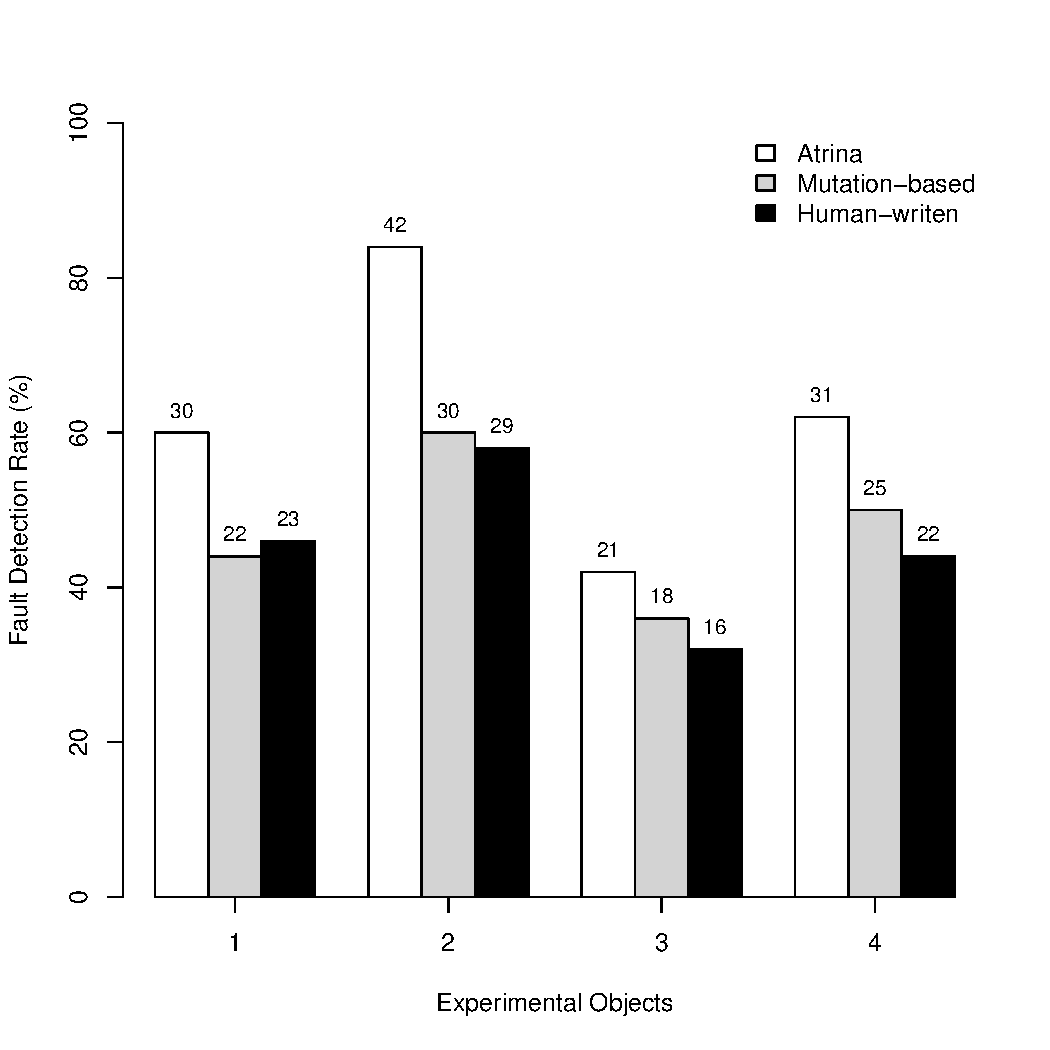
\includegraphics[width=1\hsize]{r-scripts/barplot-faultDetectionRate}
  \vspace{-0.18in}   
  \mycaption{Fault finding capability.}
  \vspace{-0.1in} 
  \label{Fig:faultDetectionRate}

\end{figure}

\headbf{Accuracy (RQ3)}
\begin{table}
        \caption{Accuracy achieved by \tool.} \label{Table:accuracyTable}        
{\scriptsize
\centering
%    \begin{center}
       
      %  \subtable[Experimental subjects and the corresponding exploration data]
            {
           \begin{tabular}{l|l|l|l|l|l} \hline
\theadturn{ID} &\theadturn{\# TP} &\theadturn{\# FP} &\theadturn{\# FN} &\theadturn{Precision (\%)} &\theadturn{Recall (\%)}  \\  \hline 

1  & 174 & 0 & 0 & 100 & 100    \\ \hline
           
2 & 861 & 18 & 162 & 98 & 84  \\ \hline

3 & 193 & 0 & 0 & 100 & 100  \\ \hline

4 & 1446 & 29 & 385 & 98 & 79 \\ \hline

\hline\end{tabular}
            }

%\end{center}
}
%\vspace{-0.2in} 
\end{table}
\headbf{Comparison with Mutation-based Assertion Generation (RQ4)}




\subsection{Threats to Validity} \label{Sec:threatsToValidity}
An external threat to the validity of our evaluation is the limited number of \javascript applications used to measure the effectiveness of our approach. We mitigated this threat by using web applications from various domains, code size, and functionality. Another threat concerns validating failed assertions through manual inspection that can be error-prone. To mitigate this threat, we carefully examine the code in which the assertion failed to make sure that the injected fault was responsible for the assertion failure. Moreover, manual computation of the \javascript slices to measure precision and recall is a time intensive task done by the authors of the paper, and thus we acknowledge that it could be error-prone, although we made every effort to mitigate this threat by precisely examining the application's code.

The regression faults we inject to evaluate the effectiveness of \tool may not be realistic. We mitigate this threat by injecting mutations that represent common \javascript applications faults, as well as using real-world web applications, and test cases written by other developers.
%\section{Discussion}
\label{Sec:discussion}

% \head{Correlation.} To examine the relationship between the 
% cyclomatic complexity of objects and the number of unique invariants, 
% we used R \cite{?} to calculate the non-parametric
% Spearman correlation coefficients (r) as well as the p-values (p), 
% and plotted the graphs. We present the combinations that
% indicate a possible correlation.\figref{inv-cc} depicts the scatter plot of the
% cyclomatic complexity versus the number of unique invariants. 
% The correlation coefficient ($r = 0.867$, $p = 0.002$) suggests that variables 
% are positively co-related: The higher the cyclomatic complexity, the more unique invariants
% are detected in the application. The reason might be that larger value of cyclomatic complexity 
% implies that more number of decision points are present in the program. Consequently, pushing more 
% restrictions on varibales and parameters of the application may result in inferring more number of
% invariants. 
% \begin{figure}
% \centering
% 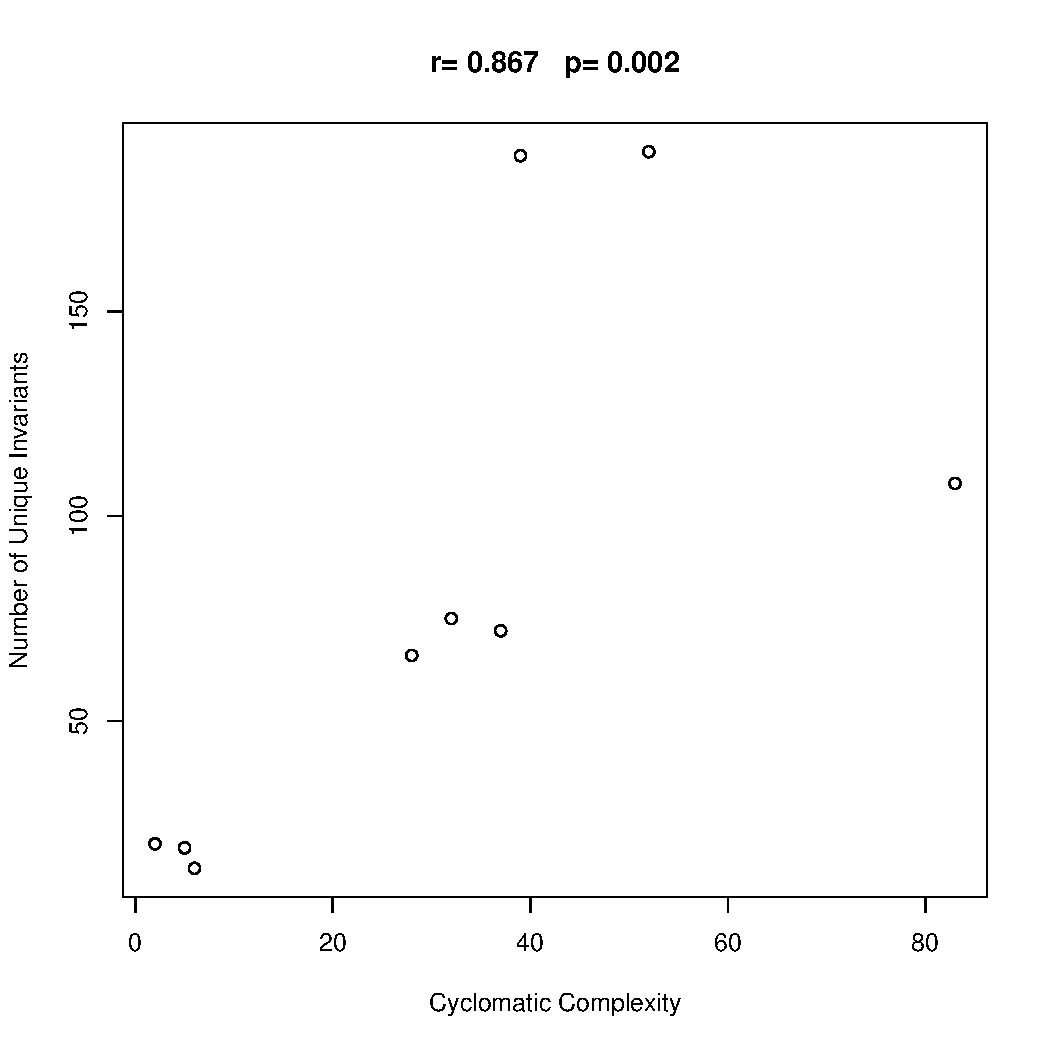
\includegraphics[width=0.7\hsize]{rscripts/inv_cc}
% \mycaption{Scatter plot of the number of unique invariants versus
% cyclomatic complexity. r represents the Spearman correlation coefficient and p is
% the p-value.}
% \label{Fig:inv-cc}
% \vspace{-0.3in}
% \end{figure}
%(1) the precision of comparing two floating point numbers in Daikon;
%The first is concerned with the number of digits in the fractional part of the floating point numbers, which is used by Daikon while comparing two floats. We resolve this by increasing the precision of float comparisons in Daikon configurations.
\head{Unstable Assertions.} As mentioned in \secref{filtering}, we observe a few number of unstable invariant assertions initially, which are removed by our filtering mechanism. By analyzing our trace data, we observe
that such unstable assertions arise mainly because of the 
multiple runtime types of \javascript variables.
This is based on the fact that in \javascript it is possible to change the type of a variable at runtime. However, Daikon treats variables as single type, selects the first observed type, and ignores the subsequent types in the trace data. This results in producing a few number of unstable invariant assertions for \javascript.
We remove such unstable assertions in our filtering step. A drawback of removing these assertions, is that our tool might miss a fault during the regression testing phase.
However, according to our observations, such unstable assertions form only around 5\% of the total generated assertions. Thus, we are still able to achieve high accuracy as presented in the previous section.
    
\head{Limitations.} Our approach is not able to detect syntax errors that are present in the \javascript code. Furthermore, tracing DOM manipulations using APIs other than the standard DOM API or jQuery is currently not supported by \jsart.
Further, a regression fault either directly violates an invariant assertion, or it can violate closely 
related assertions, which have been affected by the fault. However, if the tool is not able to infer any invariants in the  affected scope of the error, it fails to detect the fault. This results in observing a low rate of false negatives as illustrated in \secref{evaluation}. 
     
\head{Revisiting the Assumptions.} As we mentioned in \secref{approach}, we assume that the current version of the web application is bug-free. This is based on the fact that in regression testing a gold standard is always needed as a trusted version for comparing the test results against \cite{Binder:2000} to detect regression faults. However, if the original version of the application does contain an error, the generated assertions might reflect the error as well, and as such they are not able to detect the fault. 
Our second assumption states that the program specifications are unlikely to change frequently in revisions. Here we assume that software programs evolve gradually and regression faults are mostly due to small changes. However, if major upgrades occur in subsequent revisions such that the core specification of the application is affected, the inferred invariants from the original version may not be valid any longer and new invariant assertions need to be generated.

% Competent Programmer Hypothesis (CPH) \cite{acree:mutation1979, demillo:computer1978}. It states that programmers tend to develop programs, which are close to the correct version. Therefore,
% regression faults are mostly due to simple faults occur during small changes in the program. These faults made by competent programmers are merely simple faults such that the applications's behavior is not significanlty affected.


 

\begin{table}[t]
%\vspace{5pt}
        \caption{Manual effort imposed by our approach for deriving stable invariant assertions.}
{\scriptsize
    \begin{center}
       
      %  \subtable[Experimental subjects and the corresponding exploration data]
            {
           \begin{tabular}{c|c|c} \hline
\thead{App ID} & \thead{Total Time (min)} & \thead{Manual Effort (min)} \\  \hline \hline

1  & 13  & 4 \\ \hline %535
           
2  & 11.5 & 3 \\ \hline %502

3 & 15.5  & 5 \\ \hline % 639

4  & 11  & 3 \\ \hline %500

5  & 6.5 & 2.5 \\ \hline %227

6  & 9  & 4.5 \\ \hline %214

7  & 7.5  & 3.5 \\ \hline %244

8  & 6.5  & 2 \\ \hline %278

9  & 18 & 13 \\ \hline %266
\hline\end{tabular}\centering
            }
\label{Table:manualEffort_table}
\end{center}
}  
\vspace{-0.2in} 
\end{table}



\head{Automation Level.} While the testing phase of \jsart is fully automated, the navigation part requires some manual effort. Although the crawling is performed automatically, we do need to manually setup the tool with different crawling configurations per application execution.  Moreover, for each application run, we manually look at the size of the invariant output to decide whether more execution traces (and thus more crawling sessions) are needed.
%Thus, manual effort is concerned with tracing and filtering unstable invaraint assertions, where we need to execute the application 
%per crawling configuration. 
%
We present the manual effort involved with detecting stable invariant assertions in \tabref{manualEffort_table}. 
The table shows the total time, which is the duration time of deriving stable assertions including both automatic and manual parts. 
The reported manual effort contains the amount of time required 
for setting up the tool as well as the manual tasks involved with the navigation part.
The results show the average manual effort is less than 5 minutes.







  
